In recent decades, cognitive science has deepened our understanding of the mechanisms that subserve skill learning and has begun to spark ideas on how to achieve better learning by leveraging these mechanisms more effectively. Thus far, most studies have focused on simple, laboratory-based tasks, raising concerns about their applicability to real-world learning in areas such as sports, education, or rehabilitation. Therefore, there is a pressing need for studies with greater ecological validity, where learning tasks are not trivial exercises but instead improve important life functions or skills that learners genuinely care about. The overarching goal of this doctoral thesis was to bridge this gap between simple tasks and real-world skill learning with skilled performers using alpine skiing as a domain to test these theories. To achieve this goal, this doctoral thesis adopted a crossdisciplinary research approach involving mechanics and psychology. From a mechanical perspective, we asked what is the most effective strategies for skiing faster on flat slopes (aim 1) and the kinematic signatures that make one of these strategies so effective (aim 2). From a psychological perspective, we asked whether better learning effects could be achieved by applying learning theories from cognitive science to create learning problems (aim 3) and better utilize teaching signals (aim 4).  

First, we found that skiers on average achieved the fastest race times using the "extend with rock skis forward" strategy, which aligns with our expectations based on theory and quantitative field observations. This suggests that this strategy is powerful and can improve the performance of skiers on flats in slalom. However, its effect was only marginally better than that of the "extend" strategy, which is simpler and nearly as effective on its own. Based on these results, we recommend that skiers choose either of these two strategies to enhance their performance on flat sections in slalom. These findings expand upon previous ski research and provide experimental evidence for effective strategies to ski fast on flats in slalom.

Second, we also found that a training intervention focusing on the "extend" strategy left a remarkable kinematic signature on the skiers. After the intervention, skiers exhibited a more wave-like speed profile. That is, they increased their speed after passing through a gate, which continued to rise until they were approximately midway between two gates. Then, their speed decreased until the next gate, before increasing again. Additionally, we observed a trend where skiers took longer paths between gates, yet their race times improved. Together, these kinematic signatures closely resemble the predictions from Lind and Sander's model of pumping to increase velocity. A limitation of our data is that we do not know the specific movements the skiers made, preventing us from testing the model's predictions accurately. Future research should employ motion capture technology to achieve the necessary data quality for such investigations.

Shifting focus toward the testing of learning theories to improve skill learning, we did not find evidence that the skiers learned better by increasing the frequency at which they were exposed to new learning problems (that is, interleaved practice). This finding aligns with prior research that has similarly failed to observe a contextual interference effect in real-world tasks or more complex learning tasks \cite{brady_theoretical_1998, barreiros_contextual_2007, wulf_principles_2002}. Based on the results of this study and these previous findings, it may not be worthwhile to expend effort in creating multiple different slalom courses, at least concerning performance outcomes. Nonetheless, we should not dismiss the possibility that exposing skiers to rapid changes in course could influence other cognitive mechanisms. It is also plausible that the benefit of frequent course changes lies in preventing habits \cite{du_relationship_2022}, whereby skiers settle on a fixed solution and become insensitive to adapting to different situations. If so, simply changing courses sufficiently often might be adequate to avoid these habits. To better understand this phenomenon, an alternative experimental design is crucial. One approach could involve training hairpin, with one learning group practising only one hairpin while another group practising multiple hairpins.

Til slutt fant vi at å lære strategier og deres verdier gjennom med reinforcement learning var et mer effektive teaching signal enn convential instruction-based teaching with a coach.  Interestingly, the reinforcement learning group also performed descriptively better than the supervised (target skill) learning group, which was meant to serve as a benchmark for the upper limit of performance achievable through optimal strategy choices. I tillegg var effektstørrelsen av såpass størrelse at den potensielt kan ha exerted real impact on skiers world ranking based on their FIS points. Våre prediksjoner om at denne gruppeforskjellen was caused by better strategy selection on the single best strategy did not prove succesful. That is, the reinforcement learning group did not begin with or develop a greater probability of choosing the theoretically optimal strategy or the individual skier's estimated best strategy compared with the supervised (free choice) learning group. Instead, we found that the expected loss in time for skiers who made 'suboptimal' choices (that is, cost or expected regret) during the retention var lavere i reinforcement learning group than did the skiers in the supervised (free choice) learning group. One way to interpret this is that the reinforcement learning group appears to have learned to select strategies that offered comparable outcomes and to avoid those that carried the risk of substantially worse performance. One possibility is that the reinforcement learning group discovered that the "extend" strategy alone almost provided full benefits on its own and chose this strategy because it was simpler than "extend with rock skis forward". See Paper \RNum{3} for complete results and discussion.

The findings from this study suggest that reinforcement learning can serve as an effective teaching signal for selecting optimal strategies and performance. The key question is how coaches or teachers can apply this knowledge in practice. One approach is to replicate the strategies developed in the study and teach skiers to use them. However, the application can be simplified or made more advanced depending on the skill level or experience of the skiers. For less skilled skiers, learning can occur by having them ski high and low in hockey to observe the impact on their times, or by creating multiple line choices around a gate and allowing skiers to experiment with them. For more skilled skiers, a narrower set of strategies that are expected to produce smaller yet meaningful and interpretable differences can be developed. The general principle to make reinforcement learning effective is to design strategies that challenge expectations, ideally with one strategy outperforming the expected outcomes. Once skiers have established a solid understanding of the value of different strategies, it may become less useful to continue gaining experience with those strategies. At this point, coaches can either develop new sets of strategies or shift their learning strategy, such as focusing on refining the execution of the strategies. 




Avslutningsvis har jeg lyst til å evaluere den interdisiplinære tilnærmingen mellom mekanikk og psykologi for å studere skill learning in skilled athletes. 


First, some of the strategies we created based on mechanics and quantative observations of elite skiers in the field proved effective in improving skiers' race times, with some skiers improving by more than two seconds from an already high skill level. For many athletes, these strategies provided an "aha" moment. And when they realizing the power of these strateiges, they began pushing themselves further and further improved their performances. Our observations align with previous studies, which have shown that developing new strategies is crucial for continued progress. As word spread within the skiing community that our research was not just academic but genuinely improved skiers' performances, we experienced an increased interest for participating in the study. In total, we tested 186 skilled alpine skiers from Norway and Sweden, including those who served as pilot participants. All these ski teams covered their own travel and accommodation costs themselves, demonstrating the commitment and interest from the sports community. 

Fra et idrettsfaglig perspektiv er resultatene fra strategiene interessante i seg selv. Men det aller mest interessante resultatet kommer ved å trekke inn psykologi for å teste hvilket teaching signal som er mest effektive for å lære disse strategiene. Det er dette treffpunktet som har vært det unike med doktorgraden, der man lære hvilke strategier som er effektive og samtidige undersøke hvilke læringsstrategier som er mest effektive for å lære disse. Det gjør at læringseksperimentene blir så virkelighetsnært som mulig, og øker sannsynligheten for at utøvere lærer gjennom intervensjonen og at de prioriterer å bli med i prosjektet.

En utfordring med den tverrfaglige tilnærmingen er at den krever god kunnskap om både idrettens egenart og mekanikk og psykologi. Norges idrettshøgskole har vært verdenskjent for sitt gode vitenskapelige miljø på alpint der studenter har blitt godt skolert i idrettens egenart og forståelse av svingteknikk. Det er blant annet denne forståelsen av svingteknikk som vi har tuftet strategiene på. Samtidig krever den solid kunnskap om psykologi, slik at man ser disse koblingene mellom hva idretten trenger og hvilke spørsmål som psykologifaget er interessert i. Det er mange som har god kompetanse om 













Først av alt var strategiene vi lagde med forankring i mekanikk effektive for å forbedre utøveres skikjøring, og enkelte utøvere forbedret seg med over to sekunder fra et allerede høyt ferdighetsnivå. For mange utøvere ga strategiene en slags aha opplevelse. Og da det gikk opp for dem at de kunne gjøre ting annerledes og at det var mer effektive strategier enn de allerede var kjent med, prøvde de mer og forbedret sine prestasjoner ytterligere. Vår observasjon viser slående likheter med tidligere studier der man finner at utvikling av nye strategier er avgjørende for å sikre videre fremgang. Da det ble kjent i skimiljøet at utøvere ikke bare ble forsket på for forskningen sin skyld, men at strategiene faktisk forbedret utøverne sine prestasjoner var ønsket om å delta i studien stort. Totalt har vi testet 186 gode alpinister fra Norge og Sverige, inkludert skikjørere som deltok som piloter. Alle disse lagene dekket alle reise og overnattingskostnader selv, hvilket viser engasjementet og interessen fra idrettens sin side. 

Selv om man kunne gjort læringsintervensjoner på disse strategiene i seg selv er det mer 








et godt stimuli for læring.  Sikret at mange ble i prosjektet.  



tilnærmingen helt avgjørende for å oppnå fremgang hos utøvere. I begge studiene var fremgangen til utøverne i gjennomsnitt substantial, og enkelte utøvere forbedret seg med over to sekunder fra et allerede høyt nivå på den korte sekvensen. For mange ga strategiene vært en -aha opplevelse, og et godt stimuli for læring.  Sikret at mange ble i prosjektet. 




En hjørnestein for prosjektet var også den interdisiplinære tilnærmingen mellom mekanikk og psykologi, som har vært helt avgjørende for å få til fremgang hos utøvere. I begge studiene har fremgangen til utøverne vært enorm, og enkelte utøvere har forbedret seg med over to sekunder fra et allerede høyt nivå på den korte sekvensen. For mange har strategiene vært en -aha opplevelse, og et godt stimuli for læring. 




\section{Methodological considerations}



\subsection{Quantifying performance in alpine skiing}
One of the key objectives of this doctoral project was to determine a reliable method for quantifying performance in alpine skiing over time, whether over days, weeks, or months. One of the greatest challenges in this respect, from a scientific perspective, is its lack of standardization; the time taken to ski a slalom course one day may not be comparable to that of another day  Consequently, quantifying performance in alpine skiing has been widely debated, with scientists arguing for measures such as energy mechanics \cite{supej_differential_2008, supej_how_2010, supej_mechanical_2011} , differences in mechanical energy divided by time, section times \cite{supej_relations_2006}, lateral skidding of skis \cite{kirby_development_2009}, and time loss per elevation difference and distance travelled per elevation difference \cite{federolf_quantifying_2012}. Throughout my doctoral research, I have chosen to express performance in terms of time, which is the conventional way to quantify performance in skiing and allowed me to operate on the same scale as skiers and coaches do. In my doctoral reseach, I have adopted two different time measures: in papers 1 and 2, I have expressed time as the difference from the time when the skier skied the section straight down (straight gliding), whereas, in paper 3, I used the raw time to quantify performance. Here, I aim to provide some methodological reflections on these approaches to help readers evaluate the results of the studies in this doctoral thesis and to assist other researchers in the field of alpine skiing. 

To begin this methodological consideration, I conducted a Bayesian multilevel growth model on all the skiers' times as they skied straight down the section for all sessions in paper 3. From this analysis, I found that the straight gliding times for all ski groups (A, B, C, and D) increased steadily from the first session (baseline) to the last session (transfer). Although I cannot rule out any explanation for why the straight gliding times of the ski groups increased uniformly, I am confident that differences in the length of the course section are not the main explanation. This is because we used a measuring tape during the course setting, and there was a tight cluster of boreholes at the finish line, with only a few centimeters of difference. I also do not believe that changes in the skiers' starting procedures or execution of straight gliding are the main reasons. This is because the skiers were diligent and interested in performing this task as well as possible. I believe the best explanation involves the snow conditions and how we prepared them. Specifically, when grooming snow with a machine, grooves are left in the snow that becomes hard if it is watered and allowed to freeze. These hard grooves are fast to ski on because only a small part of the ski is in contact with the snow surface. As skiers complete more runs and coaches slide through the course, these snow grooves wear away, creating a smooth, hard base without grooves. When skiers descend on this groom-free base, a larger part of the ski’s contact surface touches the snow, which increases ski–snow friction and slows the skiers down.

The question is, what consequences does this have for the results, and how can we address these challenges the best possible way? First, one challenge this creates is the need to exercise caution in interpreting 'true' learning from the estimated change in race times. From From Fig. \ref{fig:rlstudy_racetime} from Study \RNum{2}, we find that the skiers improved their race times significantly over the sessions despite the increased straight gliding times. Therefore, the 'true' improvement is likely better than estimated. A less conservative and perhaps better way to express skiers' 'true' learning is to use the difference in straight gliding times for each session to account for variations in the snow surface. This is the performance measure we used in Study\RNum{1}. However, although this measure may better capture skiers' learning, we do not know whether it underestimates or overestimates learning. Another problem is that straight gliding in itself is a random variable that introduces variation and could add noise to the measurement. In Study \RNum{2}, we had to move away from this measure because the straight gliding lane crossed many holes from the previous courses. Due to these challenges, it is difficult to determine the actual improvement of skiers. Scientists therefore face two choices: either use raw race times, which is likely a conservative method that underestimates the real improvement, or express time as the difference in straight gliding, which may better account for variations in the surface and therefore express progress more accurately. The cost of the latter approach is that it underestimates or overestimates performance and could increase noise. 

Another solution is to downplay the focus on change and determine whether the learning groups differ on the postmeasure if their performance is equal at baseline, corresponding to the logic of an ANCOVA. If we have a design where skiers have undeone tests simultaneously, we can estimate this group difference, indirectly avoiding the question of change. Therefore, we used ANCOVA and raw race data in Study \RNum{2}.

One potential way to improve estimates in future research is to test more levels within the ski groups. This would allow the groups to have varying effects of the treatment and achieve better estimates through partial pooling \cite{mcelreath_statistical_2018}. We attempted to run this model, but it did not converge due to having too few levels. It might have been better to divide the ski groups into smaller subgroups that were tested at different times. This approach could have provided more levels and potentially better estimates through partial pooling. However, it must be emphasized that conducting studies such as ours is very difficult and time-consuming. Another approach is to skid extensively to eliminate the grooms before testing. 


\begin{figure}
    \centering
    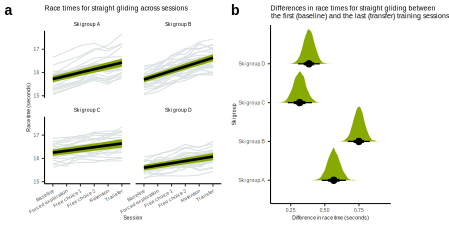
\includegraphics[width=1\linewidth]{figure/figure_methodological_straightgliding.pdf}
    \caption{Enter Caption}
    \label{fig:straightgliding}
\end{figure}